\section{Quick Start: Reducing The Demo Data \label{sec:quick_start}}

For the user who is keen on starting reductions without being
distracted by detailed documentation, we describe the steps to be
performed to reduce the science data provided in the \instname\, demo
data set 
supplied with the \reflex\ {\tt \reflexvers} release. By following these
steps, the user should have enough information to perform a reduction
of his/her own data without any further reading:

\begin{enumerate}
  \item First, type:
        \begin{verbatim}
        esoreflex -l
        \end{verbatim}

    If the \reflex\ executable is not in your path, then you have
      to provide the command with the executable full path {\tt
        <install\_dir>/bin/esoreflex -l }. For convenience, we will
      drop the reference to {\tt <install\_dir>}. A list with the
      available \reflex\ workflows will appear, showing the workflow
      names and their full path.

   \item Open the \wkfname\ by typing:

\bigskip

      {\tt \ \ \ \ \ \ \ \ esoreflex} \wkfn {\tt \&}

\bigskip

      Alternatively, you can type only the command \reflex\, the empty
      canvas will appear (Figure~\ref{fig:reflex_empty}) and you can
      select the workflow to open by clicking on {\tt File -> Open
        File}. Note that the loaded workflow will appear in a new
      window. The \wkfname\ workflow is shown in
      Figure~\ref{fig:pipe_wkf_layout}. 

  \item To aid in the visual tracking of the reduction cascade, it is advisable
  to use component (or actor) highlighting. Click on {\tt Tools -> Animate at
  Runtime}, enter the number of milliseconds representing the animation
  interval (100\,ms is recommended), and click \fbox{\tt OK}.

\item Change directories set-up. Under ``Setup Directories'' in the
  workflow canvas there are seven parameters that specify important
  directories (green dots).

  By default, the {\tt ROOT\_DATA\_DIR}, which specifies the working
  directory within which the other directories are organised. is set
  to your {\tt \$HOME/reflex\_data} directory. All the temporary and
  final products of the reduction will be organized under
  sub-directories of {\tt ROOT\_DATA\_DIR}, therefore make sure this
  parameter points to a location where there is enough disk space. To
  change {\tt ROOT\_DATA\_DIR}, double click on it and a pop-up window
  will appear allowing you to modify the directory string, which you
  may either edit directly, or use the \fbox{\tt Browse} button to
  select the directory from a file browser.  When you have finished,
  click \fbox{\tt OK} to save your changes.

    Changing the value of {\tt RAW\_DATA\_DIR} is the only necessary
    modification if you want to process data other than the demo data

  \item Click the 
  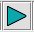
\includegraphics[width=0.5cm,height=0.5cm]{reflex_run_button.png}
  button to start the workflow

\item The workflow will highlight the {\tt Data Organiser} actor which
  recursively scans the raw data directory (specified by the parameter
  {\tt RAW\_DATA\_DIR} under ``Setup Directories'' in the workflow
  canvas) and constructs the datasets. Note that the raw and static
  calibration data must be present either in {\tt RAW\_DATA\_DIR} or
  in {\tt CALIB\_DATA\_DIR}, otherwise datasets may be incomplete and
  cannot be processed. However, if the same reference file was
  downloaded twice to different places this creates a problem as
  \reflex\ cannot decide which one to use.

\item The {\tt Data Set Chooser} actor will be highlighted next and
  will display a ``Select Datasets'' window (see
  Figure~\ref{fig:reflex_select_data_sets}) that lists the datasets
  along with the values of a selection of useful header
  keywords\footnote{The keywords listed can be changed by double
    clicking on the {\tt DataOrganiser} Actor and editing the list of
    keywords in the second line of the pop-up window. Alternatively,
    instead of double-clicking, you can press the right mouse button
    on the {\tt DataOrganiser} Actor and select {\tt Configure Actor} to
    visualize the pop-up window.}.  The first column consists of a set
  of tick boxes which allow the user to select the datasets to be
  processed. By default all complete datasets which have not yet been
  reduced will be selected. A full description of the options
    offered by the {\tt Data Set Chooser} will be presented in Section
    \ref{sec:dataset_chooser}.

  \item Click the \fbox{\tt Continue} button and watch the progress of
    the workflow by following the red highlighting of the actors. A
    window will show which dataset is currently being processed.

\ifdefined \instquickitemlist 
  \input{\instquickitemlist}
\fi

\item Once the reduction of all datasets has finished, a pop-up window
  called {\sl Product Explorer} will appear, showing the datasets
  which have been reduced together with the list of final products.
  This actor allows the user to inspect the final data products, as
  well as to search and inspect the input data used to create any of
  the products of the workflow.
  Figure~\ref{fig:reflex_provenance_explorer} shows the Product
  Explorer window.  A full description of the {\sl Product Explorer}
  will be presented in Section \ref{sec:product_explorer}.

\item After the workflow has finished, all the products from all the
  datasets can be found in a directory under {\tt END\_PRODUCTS\_DIR}
  named after the workflow start timestamp. Further subdirectories
  will be found with the name of each dataset.

\end{enumerate}

Well done! You have successfully completed the quick start section and
you should be able to use this knowledge to reduce your own
data. However, there are many interesting features of {\tt Reflex} and
the \instname\, workflow that merit a look at the rest of this tutorial.

\putgraph{8}{reflex_empty_canvas.png}{reflex_empty}{The empty {\tt
    Reflex} canvas}
